\chapter{Other Quantum Many-body Methods} \label{chp:othermethods}
\epigraph{Hartree-Fock plays the same role in many-body quantum physics as a basic kitchen tool does in cooking; it can be used to prepare almost everything.}{Morten Hjorth-Jensen}
\iffalse
\begin{figure}[H]
	\centering
	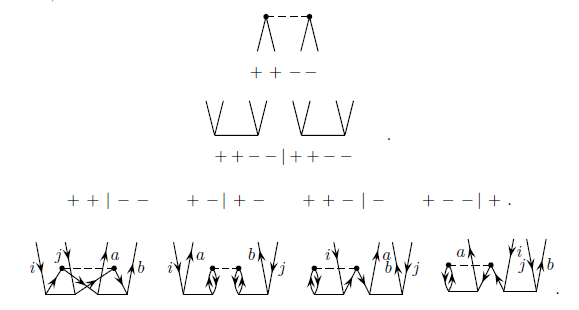
\includegraphics[scale=0.4]{Images/example.png}
	\caption{Caption}
\end{figure}
\fi

QMC methods, as presented in the previous chapter, is just a fraction of the existing many-body methods, and we will in this chapter discuss some other popular methods. Again we start from the integral representation of the Schrödinger equation, but for these methods it is a clear advantage to use Dirac notation, presented in Appendix \ref{app:dirac}. As noted in the theory, the energy eigenvalues are found from
\begin{equation}
E=\mel{\Psi}{\hat{\mathcal{H}}}{\Psi}
\end{equation}

Hartree-Fock (HF) is (arguably) the most successive many-body method, as it provides relatively accurate results with an affordable computational cost. Just a few methods give more accurate results themselves (included QMC methods), but they are in return naturally more expensive. Additionally, HF is often used as an input to other methods, which then are categorized as \textit{post Hartree-Fock methods}. Popular post Hartree-Fock methods cover the full configuration interaction method (FCI) and the coupled cluster method (CC), which both will be explained in this chapter. Also QMC methods commonly use the HF basis as inputs.

The methods HF, FCI and CC have all a fundamentally different approach to solving the Schrödinger equation compared to the QMC methods in the sense that they express the integral as expansions and require the one-body and two-body elements
\begin{equation}
\mel{\phi_i}{\hat{h}}{\phi_i}\quad\wedge\quad\mel{\phi_i\phi_j}{\hat{w}}{\phi_i\phi_j}
\end{equation}
for a given basis $\{\phi_1,\phi_2,\hdots,\phi_n\}$ in advance. $\hat{h}$ is the one-particle Hamiltonian of a particle $i$, and $\hat{w}$ is the two-particle Hamiltonian of a couple of particles $i,j$. For commonly used basis sets, these matrix elements are freely available from numerous software programs. 

The FCI method is by some considered as the most natural way of solving the Schrödinger equation, as it is a linear combination of Slater determinants yielding exact results for an infinity basis. Although this is an elegant method, it quickly becomes infeasible since it scales as $\mathcal{O}(N!)$. 

On the other hand, the CC method truncates the Slater determinants using an exponential expansion, which for an infinity basis also yields exact result. Because of the exponential treatment, the method becomes more efficient than its brother, FCI, scaling as $\mathcal{O}(N^6)$.

We have implemented the FCI and the coupled cluster doubles (CCD) algorithms, and will therefore detail the methods in the following. However, since the HF algorithm is so important, it will first be discussed thoroughly. It is implemented as well, though in its simplest form. All those methods will be applied on the atoms only as references for our VMC and RBM results.

\section{The Hartree-Fock method}
What distinguish the Hartree-Fock method from the aforementioned FCI and CC methods, is that it approximates the wave function with only \textit{one} Slater determinant. This is naturally a poorer approximations than when multiple Slater determinants are used, but on the bright side the method becomes comparably computationally cheap. The method was long called a \textit{self-consistent field method} (SCF) because electron-electron interactions are baked into the external field. However, this is not the only approach to the HF method, and it is therefore more appropriate to name the method after its inventors, Douglas Hartree and Vladimir Fock \cite{hartree_wave_1928,fock_selfconsistent_1930}. 

The idea behind the Hartree-Fock method is to include the interaction in the one-body Hamiltonian as a mean field, such that we do not need to calculate the electron-electron interaction repetitively. By introducing the Hartree-Fock operator as
\begin{equation}
\hat{h}^{\text{HF}}=\hat{t} + \hat{u}_{\text{ext}} + \hat{u}^{\text{HF}}.
\end{equation}
with $\hat{u}^{\text{HF}}$ being a single-particle potential to be determined by the HF algorithm, we can rewrite the Schrödinger equation as
\begin{equation}
\hat{h}^{\text{HF}}\ket{\psi_{\alpha}}=\varepsilon_{\alpha}\ket{\psi_{\alpha}}
\end{equation}
where $\varepsilon_{\alpha}$ is the Hartree-Fock energy and $\psi_{\alpha}$ is the single Slater determinant that provides the lowest energy. 

\subsection{The Hartree-Fock energy}
The starting point of the method is that the Hamiltonian can be split in an one-body term, $\hat{\mathcal{H}}_0$, and an interaction term, $\hat{\mathcal{H}}_{\text{I}}$, such that the energy can be expressed as
\begin{equation}
E=\mel{\Psi}{\hat{\mathcal{H}}_0}{\Psi}+\mel{\Psi}{\hat{\mathcal{H}}_{\text{I}}}{\Psi}.
\end{equation}

The one-body Hamiltonian is given by a sum over all the $N$ single-particle one-body Hamiltonians $\hat{h}_i$,
\begin{equation}
\hat{\mathcal{H}}_0=\sum_{i=1}^N\hat{h}_i=\sum_{i=1}^N\Big(\hat{t}_i+\hat{u}_i\Big)=\sum_{i=1}^N\Big(-\frac{1}{2}\nabla_i^2 + u_i\Big)
\end{equation}
as described in the preliminary quantum theory, section \ref{sec:elementary}. $\hat{t}_i$ is the kinetic energy operator of particle $i$ and $\hat{u}_i$ is the corresponding external potential operator. The one-body energy contribution is therefore commonly written as

\begin{equation}
\mel{\Psi}{\hat{\mathcal{H}}_0}{\Psi}=\sum_{i=1}^N\mel{\phi_i}{\hat{h}}{\phi_i}\equiv\sum_{i=1}^N\mel{i}{\hat{h}}{i}
\end{equation}
where we have utilized that we have one term for each $i$ and in the last expression have defined $\ket{i}\equiv\ket{\phi_i}$. 

Further, the interaction term reads
\begin{equation}
\hat{\mathcal{H}}_{\text{I}}=\sum_{i=1}^N\sum_{j>i}^N\hat{w}_{ij}=\sum_{i=1}^N\sum_{j>i}^N\frac{1}{|\bs{r}_i-\bs{r}_j|}.
\end{equation}
In order to fulfill the Pauli principle, the wave function needs to be anti-symmetric under exchange of two coordinates, and the iteraction term therefore needs to be
\begin{eqnarray}
\mel{\Psi}{\hat{\mathcal{H}}_{\text{I}}}{\Psi}=\sum_{i=1}^N\sum_{j>i}^N\Big(\mel{\phi_i\phi_j}{\hat{w}}{\phi_i\phi_j}-\mel{\phi_i\phi_j}{\hat{w}}{\phi_j\phi_i}\Big)\equiv\sum_{i=1}^N\sum_{j>i}^N\mel{ij}{\hat{w}}{ij}_{\text{AS}}
\end{eqnarray}
where we have used the short-hand notation $\ket{ij}\equiv\ket{\phi_i\phi_j}$ and the subscript, AS, implies that the element is anti-symmetric with the properties
\begin{equation}
\begin{aligned}
\mel{ij}{\hat{w}}{ij}_{\text{AS}}&=-\mel{ij}{\hat{w}}{ji}_{\text{AS}}\\
&=+\mel{ji}{\hat{w}}{ji}_{\text{AS}}\\
&=-\mel{ji}{\hat{w}}{ij}_{\text{AS}}.
\end{aligned}
\end{equation}
These relations also applies for a general matrix element $\mel{ij}{\hat{w}}{kl}_{\text{AS}}$, which is also Hermitian such that $\mel{ij}{\hat{w}}{kl}_{\text{AS}}=\mel{kl}{\hat{w}}{ij}_{\text{AS}}$.

The total energy expression is thus given by
\begin{eqnarray}
E=\sum_{i=1}^N\mel{i}{\hat{h}}{i}+\sum_{i=1}^N\sum_{j>i}^N\mel{ij}{\hat{w}}{ij}_{\text{AS}}
\end{eqnarray}
which we name the Hartree-Fock energy and which in the following will be minimized by varying the spin-orbitals $\phi_k$.

\subsection{Minimization of the Hartree-Fock energy}
Since we are replacing the interaction term, we need to define a new operator to replace the Hamiltonian, known as the Hartree-Fock operator,
\begin{equation}
\hat{h}^{\text{HF}}=\hat{t} + \hat{u}_{\text{ext}} + \hat{u}^{\text{HF}}.
\end{equation}
The $\hat{u}^{\text{HF}}$ is a single-particle potential, and will later be determined by the algorithm. The operator can be used directly in the Schrödinger equation 
\begin{equation}
\hat{h}^{\text{HF}}\ket{p}=\epsilon_{\alpha}\ket{p}
\end{equation}
where the obtained energy is called the Hartree-Fock energy. The Hartree-Fock basis is found from the following expansion,
\begin{equation}
\ket{p}=\sum_{\lambda}C_{p\lambda}\ket{\lambda},
\end{equation}
where the initial basis is denoted with Greek letters and the new basis is denoted with Roman letters. $C_{p\lambda}$ are the coefficients that form an orthogonal basis. 

When we calculated the reference energy above, our basis contained only one Slater determinant, more specifically the ground state. In Hartree-Fock, we still have a single Slater determinant basis, but we now construct new SPFs with the constraint of minimizing the energy. 

In general, one can change from one single-particle basis to another by a unitary transform,
\begin{equation}
\ket{p}=\sum_{\alpha}c_{p\alpha}\ket{\alpha},
\end{equation}
where we use greek letters for the old basis and roman letters for the new one. If we then insert into \eqref{eq:c_H_c}, we get a find energy formula with coefficients, $C_{p\lambda}$, that we can vary
\begin{equation}
E=\sum_{p}^N\sum_{\alpha\beta}C_{p\alpha}^*C_{p\beta}\mel{\alpha}{\hat{h}_0}{\beta}+\frac{1}{2}
\sum_{pq}^N\sum_{\alpha\beta\gamma\delta}C_{p\alpha}^*C_{q\beta}^*C_{p\gamma}C_{q\delta}\mel{\alpha\beta}{\hat{v}}{\gamma\delta}_{\text{AS}}.
\end{equation}
Further, we assume that also our new basis is orthonormal, i.e,
\begin{align}
	\braket{p}{q}&=\sum_{\alpha}c_{p\alpha}^*c_{q\alpha}\braket{\alpha}{\alpha}=\sum_{\alpha}c_{p\alpha}^*c_{q\alpha}=\delta_{pq}\\
	&\Rightarrow\sum_{\alpha}c_{p\alpha}^*c_{q\alpha}-\delta_{pq}=0\label{eq:constraint}
\end{align}

We now have a function, $E$, that we want to minimize with respect to a constraint given in equation \eqref{eq:constraint}. This is a typical situation where Lagrange Multipliers is convenient to use, which in this case can be written as
\begin{equation}
{\cal L}(\{C_{p\alpha}\})=E(\{C_{p\alpha}\})-\sum_a\varepsilon_a\Big(\sum_{\alpha}c_{p\alpha}^*c_{q\alpha}-\delta_{pq}\Big).
\end{equation}
The variation in reference energy is then find to be
\begin{equation}
\delta E=\sum_{k\alpha}\frac{\partial E}{\partial C_{k\alpha}^*}\delta C_{k\alpha}^*+\sum_{k\alpha}\frac{\partial E}{\partial C_{k\alpha}}\delta C_{k\alpha}-\sum_{k\alpha}\varepsilon_k(C_{k\alpha}\delta C_{k\alpha}^*+C_{k\alpha}^*\delta C_{k\alpha})
\label{eq:E_hf}
\end{equation}
which is zero when $E$ is minimized. Each coefficient $C_{k\alpha}$ and $C_{k\alpha}^*$ is independent, so they can be varied independently. Thus
\begin{equation}
\bigg(\frac{\partial E}{\partial C_{k\alpha}^*}-\varepsilon_kC_{k\alpha}\bigg)\delta C_{k\alpha}^*=0,
\end{equation}
which is satisfied if and only if
\begin{equation}
\frac{\partial E}{\partial C_{k\alpha}^*}-\varepsilon_kC_{k\alpha}=0\qquad\forall\,\,\, k,\alpha
\end{equation}
The first term can be derived from \eqref{eq:E_hf}, and reads
\begin{equation}
\frac{\partial E}{\partial C_{k\alpha}^*}=\sum_{\beta}C_{k\beta}\mel{\alpha}{\hat{h}_0}{\beta}+\sum_p^N\sum_{\beta\gamma\delta}C_{p\beta}^*C_{k\gamma}C_{p\delta}\mel{\alpha\beta}{\hat{v}}{\gamma\delta}_{\text{AS}}.
\end{equation}
This results in the equation
\begin{equation}
\sum_{\gamma}\hat{h}_{\alpha\gamma}^{\text{HF}}C_{k\gamma}=\varepsilon_kC_{k\gamma}
\label{eq:HF_sum}
\end{equation}
where we have defined
\begin{equation}
\hat{h}_{\alpha\gamma}^{\text{HF}}\equiv\mel{\alpha}{\hat{h}_0}{\gamma}+\sum_p^N\sum_{\beta\delta}C_{p\beta}^*C_{p\delta}\mel{\alpha\beta}{\hat{v}}{\gamma\delta}_{\text{AS}}.
\end{equation}
We recognize that \eqref{eq:HF_sum} can be written as a matrix-vector product
\begin{equation}
\hat{h}^{\text{HF}}C_k=\varepsilon_k^{\text{HF}}C_k
\end{equation}
where $C_k$ are columns in our coefficient matrix and $\varepsilon_k^{\text{HF}}$ are just the eigenvalues of $\hat{h}^{\text{HF}}$, they have no physical significance. We will use this equation to find the optimal SPFs (optimal $C_k$'s) and then find the energy from equation \eqref{eq:E_hf}.
\begin{equation}
\hat{h}^{\text{HF}}(C_k^{i+1})C_k^i=\varepsilon_k^{\text{HF}}C_k^i
\label{eq:HF_iter}
\end{equation}
Usually one initialize this with $\hat{C}=\hat{{\cal I}}$, the identity matrix.

\subsection{Restricted Hartree-Fock}

\subsection{Unrestricted Hartree-Fock}

\subsection{The Hartree-Fock limit}
The Hartree-Fock limit is the energy provided by the Hartree-Fock algorithm for an infinity basis set. Doing calculations with an infinity data set is obviously not possible, but we can approach the Hartree-Fock limit by using a large basis set, and there are also methods for approximating the Hartree-Fock limit even more accurate, for instance by using extrapolation. 

\section{Configuration interaction} \label{sec:ci}
The configuration interaction method is in many ways the the most intuitive method, and some will argue that it is the natural starting point. 

Often, we know the true wavefunctions $\ket{\Phi_i}$ in the external potential, but are off when interaction is added
\begin{equation}
\hat{H}_0\ket{\Phi_i}=\varepsilon_i\ket{\Phi_i},\qquad (\hat{H}_0+\hat{H}_I)\ket{\Phi_i}\neq\varepsilon_i\ket{\Phi_i}.
\end{equation}
However, the Slater determinants form a ket basis, meaning we can write out eigenstates of $\hat{H}_I$ as a linear combination of the determinants
\begin{equation}
%\begin{vmatrix}
\mqty{
	\ket{\Psi_0}&=&C_0^{(0)}\ket{\Phi_0}&+&C_1^{(0)}\ket{\Phi_1}&+&\hdots&+&C_{N-1}^{(0)}\ket{\Phi_{N-1}}\\
	\ket{\Psi_1}&=&C_0^{(1)}\ket{\Phi_0}&+&C_1^{(1)}\ket{\Phi_1}&+&\hdots&+&C_{N-1}^{(1)}\ket{\Phi_{N-1}}\\
	\ket{\Psi_2}&=&C_0^{(2)}\ket{\Phi_0}&+&C_1^{(2)}\ket{\Phi_1}&+&\hdots&+&C_{N-1}^{(2)}\ket{\Phi_{N-1}}\\
	\vdots&&\vdots&&\vdots&&&&\vdots\\
	\ket{\Psi_{N-1}}&=&C_0^{(N-1)}\ket{\Phi_0}&+&C_1^{(N-1)}\ket{\Phi_1}&+&\hdots&+&C_N^{(N-1)}\ket{\Phi_{N-1}}
}
%\end{vmatrix}
\end{equation}
such that 
\begin{equation}
\hat{H}\ket{\Psi_p}=\varepsilon_p\ket{\Psi_p}.
\end{equation}
The Hamiltonian can be rewritten as a double sum over all states using the so-called \textit{completeness relation}, 
\begin{equation}
\hat{H}=\sum_{ij}\ket{\Phi_i}\mel{\Phi_i}{\hat{H}}{\Phi_j}\bra{\Phi_j}
\end{equation}
such that the Schr\"odinger equation can be rewritten as
\begin{equation}
\begin{pmatrix}
\mel{\Phi_0}{\hat{H}}{\Phi_0} & \mel{\Phi_0}{\hat{H}}{\Phi_1} & \hdots & \mel{\Phi_0}{\hat{H}}{\Phi_{N-1}}\\
\mel{\Phi_1}{\hat{H}}{\Phi_0} & \mel{\Phi_1}{\hat{H}}{\Phi_1} & \hdots & \mel{\Phi_1}{\hat{H}}{\Phi_{N-1}}\\
\vdots & \vdots & \ddots & \vdots\\
\mel{\Phi_{N-1}}{\hat{H}}{\Phi_0} & \mel{\Phi_{N-1}}{\hat{H}}{\Phi_1} & \hdots & \mel{\Phi_{N-1}}{\hat{H}}{\Phi_{N-1}}\\
\end{pmatrix}
\begin{pmatrix}
c_0^{(p)}\\ c_1^{(p)} \\ \vdots\\ c_{N-1}^{(p)}
\end{pmatrix}
=\varepsilon_p
\begin{pmatrix}
c_0^{(p)}\\ c_1^{(p)} \\ \vdots\\ c_{N-1}^{(p)}
\end{pmatrix}
\label{eq:CIS_matrix}
\end{equation}

Until now, we have not made any assumptions, such that the equation above will give exact results when all single particle functions are included. The problem is that the matrix scales so badly, the number of Slater determinant that we need to include goes as 
\begin{equation}
N_{\text{FCI}}=\binom{N_{\text{single orbitals}}}{N_{\text{electrons}}}
\end{equation}
which is exploding. This is quite annoying since we in principle know how to solve the problems exact.

\section{Coupled Cluster} \label{subsec:cc}
The coupled cluster method is the \textit{de facto} standard wave function-based method for electronic structure calculations. \cite{paldus_beginnings_2005} The method approximates the wave function with an exponential expansion, 
\begin{equation}
\ket{\Psi_{\text{CC}}}=e^{\hat{T}}\ket{\Phi_0}
\end{equation}
where $\hatT$ is the cluster operator, entirely given by $\hatT=\hatT_1+\hatT_2 +\hatT_3+\hdots$ with
\begin{equation}
\hatT_n = \left( \frac{1}{n!}\right)^2 \sum_{abc...} \sum_{ijk...} t_{ijk...}^{abc...}a_a^\dagger a_b^\dagger a_c^\dagger \cdots a_k a_j a_i.
\end{equation}
We again want to solve the Schrödinger equation,
\begin{equation}
\hat{H}\ket{\Psi}=\hat{H}e^{\hatT}\ket{\Phi_0}=\epsilon e^{\hatT}\ket{\Phi_0},
\end{equation}
which can be simplified by multiplying with $e^{-\hatT}$ from the left. This introduces us to the \textbf{similarity transformed Hamiltonian} 
\begin{equation}
\bar{H}=e^{-\hatT}\hat{H}e^{\hatT}.
\end{equation}
If we on one hand now multiply with the reference bra on the left hand side, we easily observe that
\begin{equation}
\mel{\Phi_0}{\bar{H}}{\Phi_0}=\epsilon
\end{equation}
which is the coupled cluster energy equation. On the other hand, we can multiply with an excited bra on left hand side, and find that
\begin{equation}
\mel{\Phi_{ijk\hdots}^{abc\hdots}}{\bar{H}}{\Phi_0}=0
\end{equation}
which are the coupled cluster amplitude equations. The similarity transformed Hamiltonian can be rewritten using the Baker-Campbell-Hausdorff expansion
\begin{align}
\label{eq:BCH}
\bar{H} = \hat{H} &+ [\hat{H},\hat{T}]\notag \\
&+ \frac{1}{2}[[\hat{H},\hat{T}],\hat{T}]\notag \\
&+ \frac{1}{6}[[[\hat{H},\hat{T}],\hat{T}],\hat{T}] \\
&+ \frac{1}{24}[[[[\hat{H},\hat{T}],\hat{T}],\hat{T}],\hat{T}] \notag \\
&+ \cdots \notag
\end{align}
and we are in principle set to solve the amplitude equations with respect to the amplitudes $t_{ijk\hdots}^{abc\hdots}$ and then find the energy. The expansion is able to reproduce the true wave function exactly using a satisfying number of terms and an infinite basis. This is, of course, not possible, but even by limiting us to the first few coupled cluster operators, the results are often good compared to other methods. \cite{daniel_crawford_introduction_2007}
